%*****************************************
\chapter{Experiments}\label{ch:experiments}
%*****************************************

\section{Blocks World as a Simple Real-Time Symbolic Control Problem Domain}

\begin{figure}[bth]
  \center
  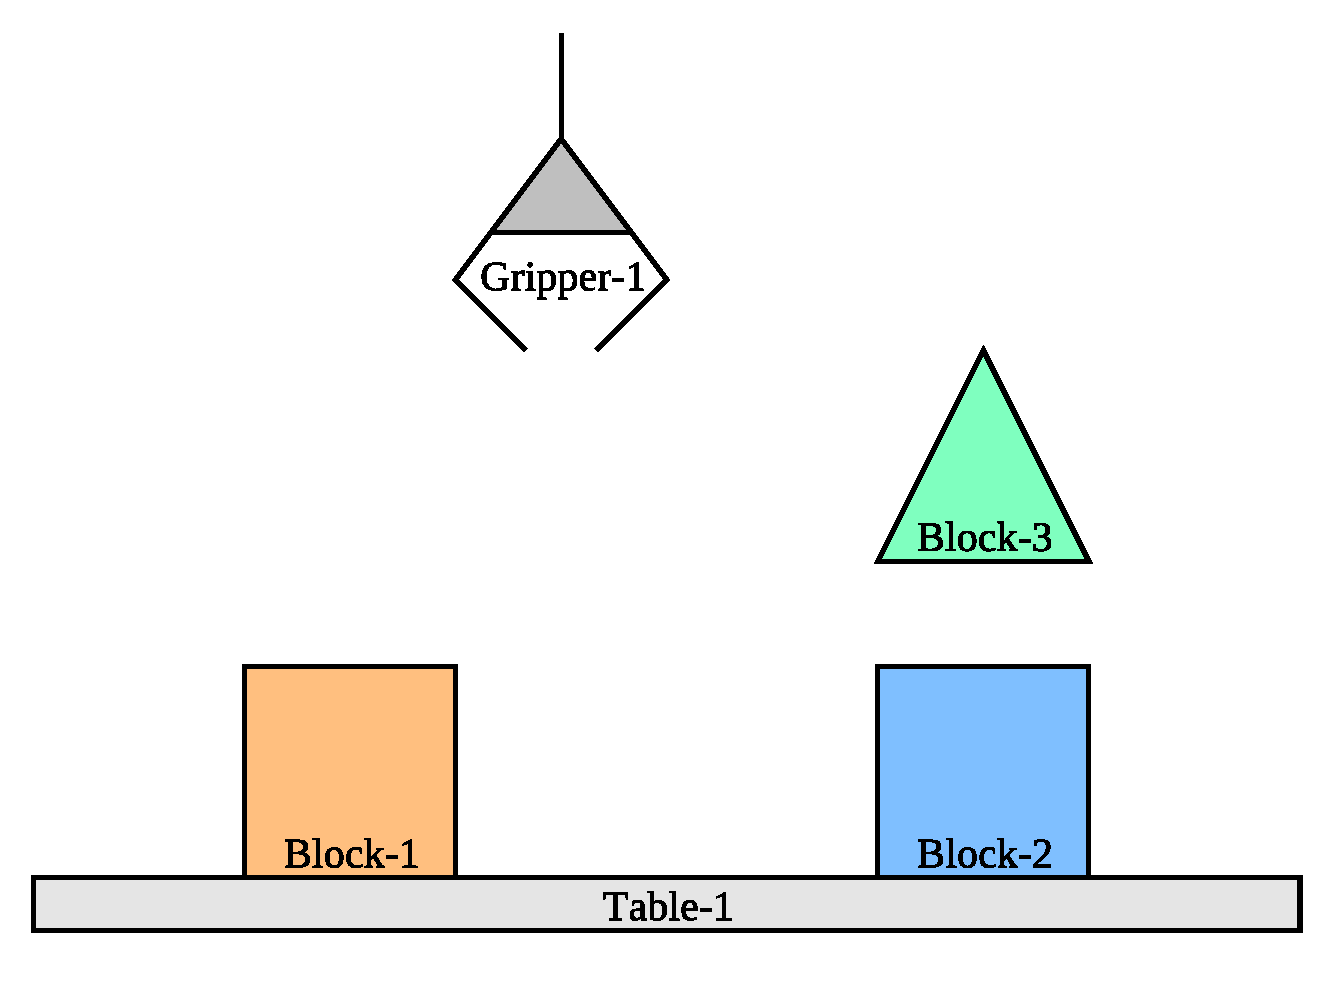
\includegraphics[width=11cm]{gfx/blocks_world_screenshot-1}
  \caption[Blocks world is a simple real-time symbolic control problem.]{Blocks world is a simple real-time symbolic control problem that we use to demonstrate our reflective control learning theory.}
  \label{fig:blocks_world_screenshot-1}
\end{figure}

I use blocks world, a canonical toy AI problem, in order to demonstrate my example of reflectively learning to plan.
See Figure~\ref{fig:blocks_world_screenshot-1} for a screenshot of my blocks world problem physical simulation.

\begin{table}
  \myfloatalign
  \begin{tabularx}{\textwidth}{XllX}
    & [Gripper-1 is me] & [Gripper-1 movement\_command []] & \\
    & [Gripper-1 is-a gripper] & [Gripper-1 color black] & \\
    & [Gripper-1 is-holding []] & [Block-1 is-a block] & \\
    & [Block-1 color brown] & [Block-1 shape cube] & \\
    & [Block-1 on Table-1] & [Block-1 left-of Gripper-1] & \\
    & [Block-2 is-a block] & [Block-2 color blue] & \\
    & [Block-2 shape cube] & [Block-2 on Table-1] & \\
    & [Block-2 right-of Gripper-1] & [Block-3 is-a block] & \\
    & [Block-3 color green] & [Block-3 shape pyramid] & \\
    & [Block-3 right-of Gripper-1] & [Table-1 is-a block] & \\
    & [Table-1 color white] & [Table-1 shape cube] & \\
    & [Table-1 left-of Gripper-1] & &
  \end{tabularx}
  \caption[Blocks world agent perceptual input.]{Blocks world agent perceptual input.}
  \label{tab:blocks_world_agent_perceptions}
\end{table}

See Table~\ref{tab:blocks_world_agent_perceptions} for an example set of perceptual input that corresponds with the physical situation shown in Figure~\ref{fig:blocks_world_screenshot-1}.

\section{Working in a World of Building Blocks}

In his PhD thesis, Terry Winograd worked in the world of building
blocks \citep{winograd:1970}.  This program maintained traces of its
goals and subgoals, which enabled it to answer questions about why it
performed certain actions.  This system worked because it stored
goals.

Knowing the goal state of the computation is important, and we do not
ignore this aspect in tracing the deliberative layer.  Our system is
able to answer these sorts of questions, as this simply requires
climbing the stack of mental resource activations, but when debugging
the deliberative process, it is helpful to not only know the ending
point of computation but also the means toward that end.

\section{Terry Winograd's SHRDLU and Goal Tracing}

I am building upon what was learned from Winograd's thesis
\citep{winograd:1970} in terms of using traces of the deliberative
process as well as using a semantic model of the world in order to
understand communications between agents.  I have chosen to use a
simpler and more direct language interface between agents that refers
more directly to the semantic information and mental processes
involved.

\section{Why Not Work Within a Building Blocks Domain?}

The building blocks approach is a good precedent.  I did not want to
get buried in the morass of common sense knowledge problems about
cooking, but I did want to approach a domain in which there are a
variety of objects requiring complex models of cause and effect.

We have conscripted our domain of object types in the kitchen, such
that it is currently comparable to the number of object types that
Winograd used in his thesis.  Our object types do have different ways
that they may be used, which is a small addition of complexity.
Although we do not introduce many of the complexities of ontological
reasoning, a common approach to commonsense reasoning, e.g. Cyc
\citep{lenat:1990}, our system demonstrates an important new approach
to commonsense reasoning that grounds learning by being told in the
domain of goal-oriented reasoning, which allows organizing and
debugging knowledge in terms of what goals it is useful for
accomplishing.

\section{A Demonstration in a Social Commonsense Reasoning Domain}

The goal of our project is to build a demo of part of Minsky's
architecture, and the domain of commonsense reasoning in a kitchen is
I feel the right way to develop those high-level theories.

We tested our cognitive architecture learning in the context of a
social commonsense reasoning domain with parents that teach children
as they attempt to accomplish cooking tasks in a kitchen.  Kitchens
are a good example of a rich learning environment for children
\citep{dewey:1907}.  Kitchens are ubiquitous across cultures.  They
have a clear production goal, food.  They involve many many mental
realms: math, physics, chemistry, thermodynamics, natural language,
social, family, imprimer learning, children, parents, concurrent
planning, etc.

